\documentclass[10pt]{beamer}

% ------------------------------------------------------------------------
% Carga de tu preámbulo personalizado (preamble.tex).
% Asegúrate de tenerlo en la misma carpeta para que \input funcione.
% ------------------------------------------------------------------------
\usetheme[progressbar=frametitle]{metropolis}
\usepackage{appendixnumberbeamer}
\usepackage{fancyvrb}
\usepackage{booktabs}
\usepackage[scale=2]{ccicons}
\usepackage{pgfplots}
\usepgfplotslibrary{dateplot}
\usepackage{type1cm}
\usepackage{lettrine}
\usepackage{ragged2e}
\usepackage{xspace}
\newcommand{\themename}{\textbf{\textsc{metropolis}}\xspace}
\usepackage{graphicx} % Allows including images
\usepackage{booktabs} % Allows the use of \toprule, \midrule and \bottomrule in tables
\usepackage[utf8]{inputenc} %solucion del problema de los acentos.
\usepackage{xcolor}
\definecolor{LightGray}{gray}{0.9}

\usepackage{minted}
\usemintedstyle{tango}
\newcommand{\mypyfile}[1]{\inputminted[linenos=true, fontsize=\footnotesize, frame=lines, framesep=5\fboxrule,framerule=1pt]{python}{#1}}

\setminted[python]{breaklines,frame=lines,framesep=2mm,baselinestretch=1.2,bgcolor=LightGray,linenos, fontsize=\footnotesize} % obeytabs=true, tabsize=2, showtabs=true}

%%%%%%%%%%%%%%%%%%%%%%%%%%%%%%%%%%%%%%%%%%%%%%%%%%%%%%%%%%%%%%%%%%%%%%%%%%%%%%%%%%%%%%
\setbeamercolor{progress bar}{fg=blue!50!black,bg=white!50!black}
\setbeamercolor{title separator}{fg=red!50!black,bg=white!50!black}
\setbeamercolor{frametitle}{fg=white!80!black,bg=red!50!black}
\title[PCFI161]{Programaci\'on para F\'isica y Astronom\'ia}
\subtitle{Departamento de Física.}

\newcommand{\myfront}{
\author[PCFI161]{Corodinadora: C Loyola \\ Profesoras/es C Loyola / C Femenías / Y Navarrete / C Ruiz}
\institute[UNAB]{Universidad Andrés Bello}
\date{Primer Semestre 2025}
}

\titlegraphic{%
  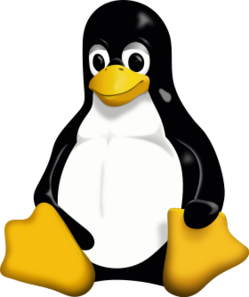
\includegraphics[width=.08\textwidth]{logo-tux.png}\hfill
  
\includegraphics[width=.3\textwidth]{logo-unab.png}\hfill
  
\includegraphics[width=.08\textwidth]{logo-python.png}
}

\makeatletter
\setbeamertemplate{title page}{
  \begin{minipage}[b][\paperheight]{\textwidth}
    \vfill%
    \ifx\inserttitle\@empty\else\usebeamertemplate*{title}\fi
    \ifx\insertsubtitle\@empty\else\usebeamertemplate*{subtitle}\fi
    \usebeamertemplate*{title separator}
    \ifx\beamer@shortauthor\@empty\else\usebeamertemplate*{author}\fi
    \ifx\insertdate\@empty\else\usebeamertemplate*{date}\fi
    \ifx\insertinstitute\@empty\else\usebeamertemplate*{institute}\fi
    \vfill
    \ifx\inserttitlegraphic\@empty\else\inserttitlegraphic\fi
    \vspace*{1cm}
  \end{minipage}
}
\makeatother


\makeatletter
\setlength{\metropolis@titleseparator@linewidth}{2pt}
\setlength{\metropolis@progressonsectionpage@linewidth}{2pt}
\setlength{\metropolis@progressinheadfoot@linewidth}{2pt}
\makeatother


\begin{document}

% ------------------------------------------------------------------------
% Portada de la Presentación
% ------------------------------------------------------------------------
\myfront{}

% ------------------------------------------------------------------------
% Slide 1: Título de la Sesión
% ------------------------------------------------------------------------
\begin{frame}
  \titlepage
  % Por ejemplo:
  % \title{Semana 6 - Sesión 1 (Sesión 11): Introducción a la Biblioteca NumPy}
\end{frame}

% ------------------------------------------------------------------------
% Slide 2: Índice / Tabla de Contenidos
% ------------------------------------------------------------------------
\begin{frame}
  \frametitle{Resumen - Semana 6, Sesión 1 (Sesión 11)}
  \tableofcontents
\end{frame}

% ------------------------------------------------------------------------
% Configuración de bloques (en caso de usar metrópolis, etc.)
% ------------------------------------------------------------------------
\metroset{block=fill}

% ----------------------------------------------------------------------------------------
% SECCIÓN 1: Introducción y Conexión con la Sesión Anterior
% ----------------------------------------------------------------------------------------
\section{Introducción y Contexto}

% ------------------------------------------------------------------------
% Slide 3: Retorno tras la Solemne
% ------------------------------------------------------------------------
\begin{frame}{Después de la Solemne I}
  \begin{itemize}
    \item \textbf{Semana 5} incluyó un repaso integral y la \textbf{Solemne I}.
    \item Ahora retomamos contenidos para profundizar nuestras habilidades de programación.
    \item \textbf{Objetivo de esta sesión}: Introducir la librería \textbf{NumPy} para manejo eficiente de arreglos y cálculos numéricos.
  \end{itemize}
\end{frame}

% ------------------------------------------------------------------------
% Slide 4: Objetivos de la Sesión 11
% ------------------------------------------------------------------------
\begin{frame}{Objetivos de la Sesión 11}
  \begin{itemize}
    \item \textbf{Comprender} los conceptos básicos de NumPy: arreglos (arrays), vectorización, broadcasting.
    \item \textbf{Practicar} la creación y manipulación de arrays en Google Colab.
    \item \textbf{Aplicar} estas herramientas a ejemplos numéricos y pequeños problemas de Física/Astronomía.
    \item \textbf{Fomentar} la colaboración y el trabajo práctico en laboratorio.
  \end{itemize}
\end{frame}

% ----------------------------------------------------------------------------------------
% SECCIÓN 2: ¿Por qué NumPy?
% ----------------------------------------------------------------------------------------
\section{Motivación: NumPy}

% ------------------------------------------------------------------------
% Slide 5: ¿Qué es NumPy?
% ------------------------------------------------------------------------
\begin{frame}{¿Qué es NumPy?}
  \begin{itemize}
    \item \textbf{NumPy} = \textbf{Num}erical \textbf{Py}thon.
    \item Ofrece:
      \begin{itemize}
        \item Estructura central: \textbf{ndarray} (arreglo multidimensional).
        \item Funciones matemáticas optimizadas para operar sobre estos arreglos.
        \item Alto rendimiento (implementaciones en C bajo la interfaz de Python).
      \end{itemize}
    \item \textbf{Base de muchas librerías} científicas (p.e. SciPy, Pandas, etc.).
  \end{itemize}
\end{frame}

% ------------------------------------------------------------------------
% Slide 6: Ventajas Frente a Listas de Python
% ------------------------------------------------------------------------
\begin{frame}{Ventajas frente a Listas Nativas de Python}
  \begin{itemize}
    \item \textbf{Vectorización}: escribir operaciones como \texttt{arr * 2} en lugar de bucles manuales.
    \item \textbf{Rendimiento}: implementaciones de bajo nivel (C/Fortran) para cálculos numéricos.
    \item \textbf{Herramientas avanzadas}: slicing sofisticado, broadcasting, manipulación de ejes (dimensiones).
    \item \textbf{Compatibilidad} con otras librerías (Matplotlib, SciPy, etc.).
  \end{itemize}
\end{frame}

% ----------------------------------------------------------------------------------------
% SECCIÓN 3: Primeros Pasos con NumPy
% ----------------------------------------------------------------------------------------
\section{Primeros Pasos con NumPy}

% ------------------------------------------------------------------------
% Slide 7: Instalación y Importación
% ------------------------------------------------------------------------
\begin{frame}[fragile]{Instalación y Importación}
  \begin{itemize}
    \item En muchos entornos (Colab, Anaconda), NumPy ya está incluido.
    \item Si fuera necesario:
\begin{minted}{bash}
pip install numpy
\end{minted}
    \item \textbf{Importación típica}:
\begin{minted}{python}
import numpy as np
\end{minted}
    \item A partir de ahí, usamos \texttt{np.array}, \texttt{np.mean}, etc.
  \end{itemize}
\end{frame}

% ------------------------------------------------------------------------
% Slide 8: Creación de Arrays
% ------------------------------------------------------------------------
\begin{frame}[fragile]{Creación de Arrays NumPy}
\begin{minted}[
  frame=lines,
  framesep=2mm,
  bgcolor=LightGray,
  fontsize=\footnotesize
]{python}
import numpy as np

# Convertir lista de Python a array NumPy
lista = [1, 2, 3, 4]
arr = np.array(lista)
print("Array:", arr)
print("Tipo:", type(arr))  # <class 'numpy.ndarray'>

# Array de ceros
zeros = np.zeros(5)
print("Zeros:", zeros)

# Array de unos
unos = np.ones((2,3))  # 2 filas x 3 columnas
print("Unos:\n", unos)

# Rango de valores
rango = np.arange(0, 10, 2)  # [0, 2, 4, 6, 8]
\end{minted}
\end{frame}

% ------------------------------------------------------------------------
% Slide 9: Atributos de un Array
% ------------------------------------------------------------------------
\begin{frame}[fragile]{Atributos de un Array}
\begin{minted}[
  frame=lines,
  framesep=2mm,
  bgcolor=LightGray,
  fontsize=\footnotesize
]{python}
arr = np.array([[1, 2, 3],
                [4, 5, 6]])
print("Shape:", arr.shape)   # (2, 3)
print("Dim:", arr.ndim)      # 2
print("Tipo de datos:", arr.dtype)  # int64 (en sistemas Linux)
print("Total de elementos:", arr.size) # 6
\end{minted}
\begin{itemize}
  \item \texttt{shape} = tupla de dimensiones.
  \item \texttt{dtype} = tipo de dato (\texttt{int32, float64}, etc.).
  \item \texttt{ndim} = número de ejes.
\end{itemize}
\end{frame}

% ----------------------------------------------------------------------------------------
% SECCIÓN 4: Manipulación y Operaciones
% ----------------------------------------------------------------------------------------
\section{Manipulación de Arrays y Operaciones}

% ------------------------------------------------------------------------
% Slide 10: Slicing y Indexación
% ------------------------------------------------------------------------
\begin{frame}[fragile]{Slicing e Indexación}
\begin{minted}[
  frame=lines,
  framesep=2mm,
  bgcolor=LightGray,
  fontsize=\footnotesize
]{python}
arr = np.array([10, 20, 30, 40, 50])
print(arr[0])      # 10
print(arr[1:3])    # [20 30]

mat = np.array([[1, 2, 3],
                [4, 5, 6],
                [7, 8, 9]])
# Acceder a fila 1, columna 2
print(mat[1, 2])   # 6

# Slicing de filas y columnas
submat = mat[0:2, 1:3]  # Filas [0..1], Cols [1..2]
print(submat)
\end{minted}
\begin{itemize}
  \item \textbf{Ojo}: en NumPy, slicing crea \textbf{vistas}, no copias (con implicaciones en la modificación de datos).
\end{itemize}
\end{frame}

% ------------------------------------------------------------------------
% Slide 11: Operaciones Elemento a Elemento
% ------------------------------------------------------------------------
\begin{frame}[fragile]{Operaciones Elemento a Elemento (Vectorización)}
\begin{minted}[
  frame=lines,
  framesep=2mm,
  bgcolor=LightGray,
  fontsize=\footnotesize
]{python}
x = np.array([1, 2, 3])
y = np.array([4, 5, 6])

print("Suma:", x + y)   # [5  7  9]
print("Producto:", x * y)  # [4 10 18]
print("Potencia:", x**2)   # [1 4 9]
\end{minted}
\begin{itemize}
  \item \textbf{Sin} bucles explícitos.
  \item El núcleo de NumPy optimiza estas operaciones.
\end{itemize}
\end{frame}

% ------------------------------------------------------------------------
% Slide 12: Broadcasting
% ------------------------------------------------------------------------
\begin{frame}[fragile]{Broadcasting}
  \begin{itemize}
    \item Mecanismo que NumPy utiliza para manejar operaciones entre arrays de diferentes formas.
    \item \textbf{Ejemplo}:
\begin{minted}[
  frame=lines,
  framesep=2mm,
  fontsize=\footnotesize,
  bgcolor=LightGray
]{python}
a = np.array([1, 2, 3])
b = 2
# b se "expande" para coincidir con la forma de a
res = a * b  # [2 4 6]
\end{minted}
    \item También puede ocurrir con arreglos 2D y 1D, etc.
  \end{itemize}
\end{frame}

% ------------------------------------------------------------------------
% Slide 13: Ejemplo de Broadcasting Matricial
% ------------------------------------------------------------------------
\begin{frame}[fragile]{Ejemplo: Sumar Fila a una Matriz}
\begin{minted}[
  frame=lines,
  framesep=2mm,
  fontsize=\footnotesize,
  bgcolor=LightGray
]{python}
mat = np.array([[1,2,3],
                [4,5,6],
                [7,8,9]])
fila = np.array([10, 20, 30])

# Broadcasting: se suma fila a cada fila de la matriz
res = mat + fila
print(res)
# [[11 22 33]
#  [14 25 36]
#  [17 28 39]]
\end{minted}
\begin{itemize}
  \item NumPy reconoce que \texttt{fila} es de 1D y la "extiende" sobre las filas.
\end{itemize}
\end{frame}

% ----------------------------------------------------------------------------------------
% SECCIÓN 5: Operaciones Numéricas y Práctica
% ----------------------------------------------------------------------------------------
\section{Operaciones Numéricas y Práctica}

% ------------------------------------------------------------------------
% Slide 14: Funciones NumPy Comunes
% ------------------------------------------------------------------------
\begin{frame}[fragile]{Funciones NumPy Comunes}
\begin{minted}[
  frame=lines,
  framesep=2mm,
  fontsize=\footnotesize,
  bgcolor=LightGray
]{python}
arr = np.array([2, 4, 6, 8])

print("Suma total:", np.sum(arr))           # 20
print("Mínimo:", np.min(arr))              # 2
print("Máximo:", np.max(arr))              # 8
print("Promedio:", np.mean(arr))           # 5.0
print("Desv. Estándar:", np.std(arr))       # ~2.236
\end{minted}
\begin{itemize}
  \item También hay \texttt{np.median(arr)}, \texttt{np.var(arr)} y muchas más.
  \item Para arreglos 2D, se puede especificar \texttt{axis=0} o \texttt{axis=1}.
\end{itemize}
\end{frame}

% ------------------------------------------------------------------------
% Slide 15: Ejercicio 1 - Primer Contacto con NumPy
% ------------------------------------------------------------------------
\begin{frame}{Ejercicio 1: Primer Contacto con NumPy}
  \begin{block}{Enunciado}
    \begin{itemize}
      \item Crear un arreglo 1D con los números del 1 al 10.
      \item Imprimir su \textbf{media}, \textbf{suma} y \textbf{producto} de todos los elementos.
      \item Reemplazar los valores \(\leq 5\) por 0, y los restantes por 1 (opcional: slicing lógico).
      \item Mostrar el arreglo resultante.
    \end{itemize}
  \end{block}
  \textbf{Sugerencia}: Usa \texttt{np.arange} y \textbf{operaciones de comparación} (\texttt{arr <= 5}).
\end{frame}

% ------------------------------------------------------------------------
% Slide 16: Ejercicio 2 - Matriz y Broadcasting
% ------------------------------------------------------------------------
\begin{frame}{Ejercicio 2: Matriz y Broadcasting}
  \begin{block}{Enunciado}
    \begin{itemize}
      \item Crear una matriz 3x3 con \(\{[1,2,3],[4,5,6],[7,8,9]\}\).
      \item Definir un \textbf{vector} \([10, 20, 30]\).
      \item Sumar dicho vector a cada fila de la matriz (broadcasting).
      \item Mostrar el resultado.
    \end{itemize}
  \end{block}
  \textbf{Objetivo}: Practicar la manipulación 2D y la “extensión” de forma con un vector 1D.
\end{frame}

% ------------------------------------------------------------------------
% Slide 17: Ejercicio 3 - Pequeño Desafío Numérico
% ------------------------------------------------------------------------
\begin{frame}{Ejercicio 3: Aproximación de \(\pi\) con Serie}
  \begin{block}{Enunciado}
    \begin{itemize}
      \item Usar \texttt{np.arange} para generar un rango de \texttt{n} valores.
      \item Calcular una aproximación de \(\pi\) usando la serie de Leibniz:
      \[
        \pi \approx 4 \sum_{k=0}^{n} \frac{(-1)^k}{2k+1}
      \]
      \item Comparar el valor obtenido para distintos \texttt{n}.
    \end{itemize}
  \end{block}
  \textbf{Sugerencia}: Emplear \textbf{vectorización} para computar \(\frac{(-1)^k}{2k+1}\).
\end{frame}

% ------------------------------------------------------------------------
% Slide 18: Trabajo en Grupos (Laboratorio)
% ------------------------------------------------------------------------
\begin{frame}{Trabajo en Grupos}
  \begin{itemize}
    \item Dividir la clase en \textbf{parejas o tríos}.
    \item Resolver los ejercicios en un \textbf{notebook de Colab}.
    \item Explorar ejemplos adicionales: 
      \begin{itemize}
        \item Generar \textbf{matrices aleatorias} (\texttt{np.random.rand()}) y calcular su determinante (\textbf{opcional, con \texttt{np.linalg.det}}).
        \item Practicar slicing y reemplazo de submatrices.
      \end{itemize}
  \end{itemize}
\end{frame}

% ------------------------------------------------------------------------
% Slide 19: Espacio para Dudas
% ------------------------------------------------------------------------
\begin{frame}{Espacio para Dudas}
  \begin{itemize}
    \item ¿Problemas de instalación o importación en Colab?
    \item ¿Dificultad para entender la forma \texttt{(shape)} de un arreglo?
    \item ¿Alguna confusión con slicing, vistas y copias?
  \end{itemize}
  \vspace{0.3cm}
  \textbf{Comparte tus dudas o experiencias, discutimos en conjunto.}
\end{frame}

% ------------------------------------------------------------------------
% Slide 20: Ejemplo de Solución (Ejercicio 1)
% ------------------------------------------------------------------------
\begin{frame}[fragile]{Ejemplo: Solución Ejercicio 1}
\begin{minted}[
  frame=lines,
  framesep=2mm,
  fontsize=\footnotesize,
  bgcolor=LightGray
]{python}
import numpy as np

arr = np.arange(1, 11)  # [1..10]
print("Array:", arr)

print("Media:", np.mean(arr))   # 5.5
print("Suma:", np.sum(arr))     # 55
print("Producto:", np.prod(arr))# 3628800

# Reemplazo valores <=5 con 0, y >5 con 1
arr_mod = arr.copy()
arr_mod[arr_mod <= 5] = 0
arr_mod[arr_mod > 5] = 1
print("Array modificado:", arr_mod)
\end{minted}
\end{frame}

% ------------------------------------------------------------------------
% Slide 21: Ejemplo de Solución (Ejercicio 2)
% ------------------------------------------------------------------------
\begin{frame}[fragile]{Ejemplo: Solución Ejercicio 2}
\begin{minted}[
  frame=lines,
  framesep=2mm,
  fontsize=\footnotesize,
  bgcolor=LightGray
]{python}
import numpy as np

mat = np.array([[1,2,3],
                [4,5,6],
                [7,8,9]])
fila = np.array([10, 20, 30])

resultado = mat + fila  # Broadcasting
print("Matriz resultante:\n", resultado)
# [[11 22 33]
#  [14 25 36]
#  [17 28 39]]
\end{minted}
\end{frame}

% ------------------------------------------------------------------------
% Slide 22: Ejemplo de Solución (Ejercicio 3)
% ------------------------------------------------------------------------
\begin{frame}[fragile]{Ejemplo: Solución Ejercicio 3 (Leibniz \(\pi\))}
\begin{minted}[
  frame=lines,
  framesep=2mm,
  fontsize=\footnotesize,
  bgcolor=LightGray
]{python}
import numpy as np

n = 100000  # término superior
k = np.arange(n+1)  # [0..n]

# (-1)^k = np.power(-1, k)
# denominador = (2*k + 1)
terminos = ((-1)**k) / (2*k + 1)
aprox_pi = 4 * np.sum(terminos)
print("Aproximación de pi con n =", n, ":", aprox_pi)

# Comparar con valor real
import math
print("Diferencia:", abs(math.pi - aprox_pi))
\end{minted}
\end{frame}

% ------------------------------------------------------------------------
% Slide 23: Discusión de Resultados
% ------------------------------------------------------------------------
\begin{frame}{Discusión de Resultados}
  \begin{itemize}
    \item \textbf{Verificación}: ¿Coincidió con tus resultados o surgieron discrepancias?
    \item \textbf{Rendimiento}: usar vectorización en lugar de bucles manuales.
    \item \textbf{Optimización}: manipulación y slicing evitan copias innecesarias.
  \end{itemize}
\end{frame}

% ----------------------------------------------------------------------------------------
% SECCIÓN 6: Conclusiones y Próximos Pasos
% ----------------------------------------------------------------------------------------
\section{Conclusiones y Próximos Pasos}

% ------------------------------------------------------------------------
% Slide 24: Conclusiones de la Sesión 11
% ------------------------------------------------------------------------
\begin{frame}{Conclusiones de la Sesión 11}
  \begin{itemize}
    \item Entendimos la importancia de \textbf{NumPy} para cálculos numéricos y arreglos multidimensionales.
    \item Practicamos \textbf{creación}, \textbf{slicing}, \textbf{operaciones vectorizadas} y \textbf{broadcasting}.
    \item Vimos ejemplos de aplicación en problemas matemáticos y de simulación.
    \item Próximamente, profundizaremos en \textbf{manipulación avanzada} de datos y su visualización (Matplotlib, etc.).
  \end{itemize}
\end{frame}

% ------------------------------------------------------------------------
% Slide 25: Próxima Sesión
% ------------------------------------------------------------------------
\begin{frame}
  \Huge{\centerline{¡Gracias por su atención!}}
  \vspace{0.3cm}
  \normalsize
  \begin{itemize}
    \item En la \textbf{próxima sesión} (Semana 6, Sesión 2) exploraremos más operaciones avanzadas con NumPy (reshaping, funciones linalg, etc.) y su integración con \textbf{Matplotlib}.
    \item ¡Sigan practicando con los ejercicios y datos reales para asimilar mejor NumPy!
  \end{itemize}
\end{frame}

\end{document}

